% ======================================================
% Configuration Manual – N-of-1 ADHD + Bipolar Disorder
% Practicum Part 2 – MSc Artificial Intelligence for Business
% National College of Ireland – Rodrigo Marques Teixeira
% ✅ This template targets **pdfLaTeX** (Overleaf default) and avoids engine‑specific packages.
% ======================================================

\documentclass[12pt,a4paper]{article}

% ---------- Packages (pdfLaTeX‑safe) ----------
\usepackage[utf8]{inputenc}
\usepackage[T1]{fontenc}
\usepackage{lmodern}
\usepackage{microtype}
\usepackage{geometry}
\usepackage{graphicx}
\usepackage{booktabs}
\usepackage{longtable}
\usepackage{float}
\usepackage{caption}
\usepackage{hyperref}
\usepackage{amsmath, amssymb}
\usepackage{xcolor}

% ---------- Layout ----------
\geometry{margin=2.5cm}
\setlength{\parskip}{0.6em}
\setlength{\parindent}{0pt}
\hypersetup{
  colorlinks=true,
  linkcolor=blue,
  urlcolor=blue,
  citecolor=blue,
  pdfauthor={Rodrigo Marques Teixeira},
  pdftitle={Configuration Manual (Full) – N-of-1 ADHD + BD}
}

% ---------- Title ----------
\title{\textbf{Configuration Manual (Full Version)}\\N-of-1 Study – ADHD + Bipolar Disorder\\\vspace{0.4cm}\large Practicum Part 2 – MSc in Artificial Intelligence for Business}
\author{\textbf{Rodrigo Marques Teixeira} \\ National College of Ireland \\ Supervisor: Dr. Agatha Mattos}
\date{October 2025}

\begin{document}
\maketitle
\tableofcontents
\newpage

% ======================================================
% 1. Introduction
% ======================================================
\section{Introduction}
This manual documents the configuration and reproducibility details for Practicum Part 2. It covers ETL, modeling, explainability, and ethical governance for the N-of-1 longitudinal study on ADHD and Bipolar Disorder.

% ======================================================
% 2. System Architecture
% ======================================================
\section{System Architecture}
\textbf{Components:} data sources (Apple Health, Amazfit GTR4, Helio Ring, EMA), ETL pipeline, modeling notebooks, and SHAP explainability. Include a simple block diagram as a figure (PNG/PDF) placed under \texttt{docs/figures/} and referenced with \verb|\includegraphics|.

\begin{figure}[H]
  \centering
  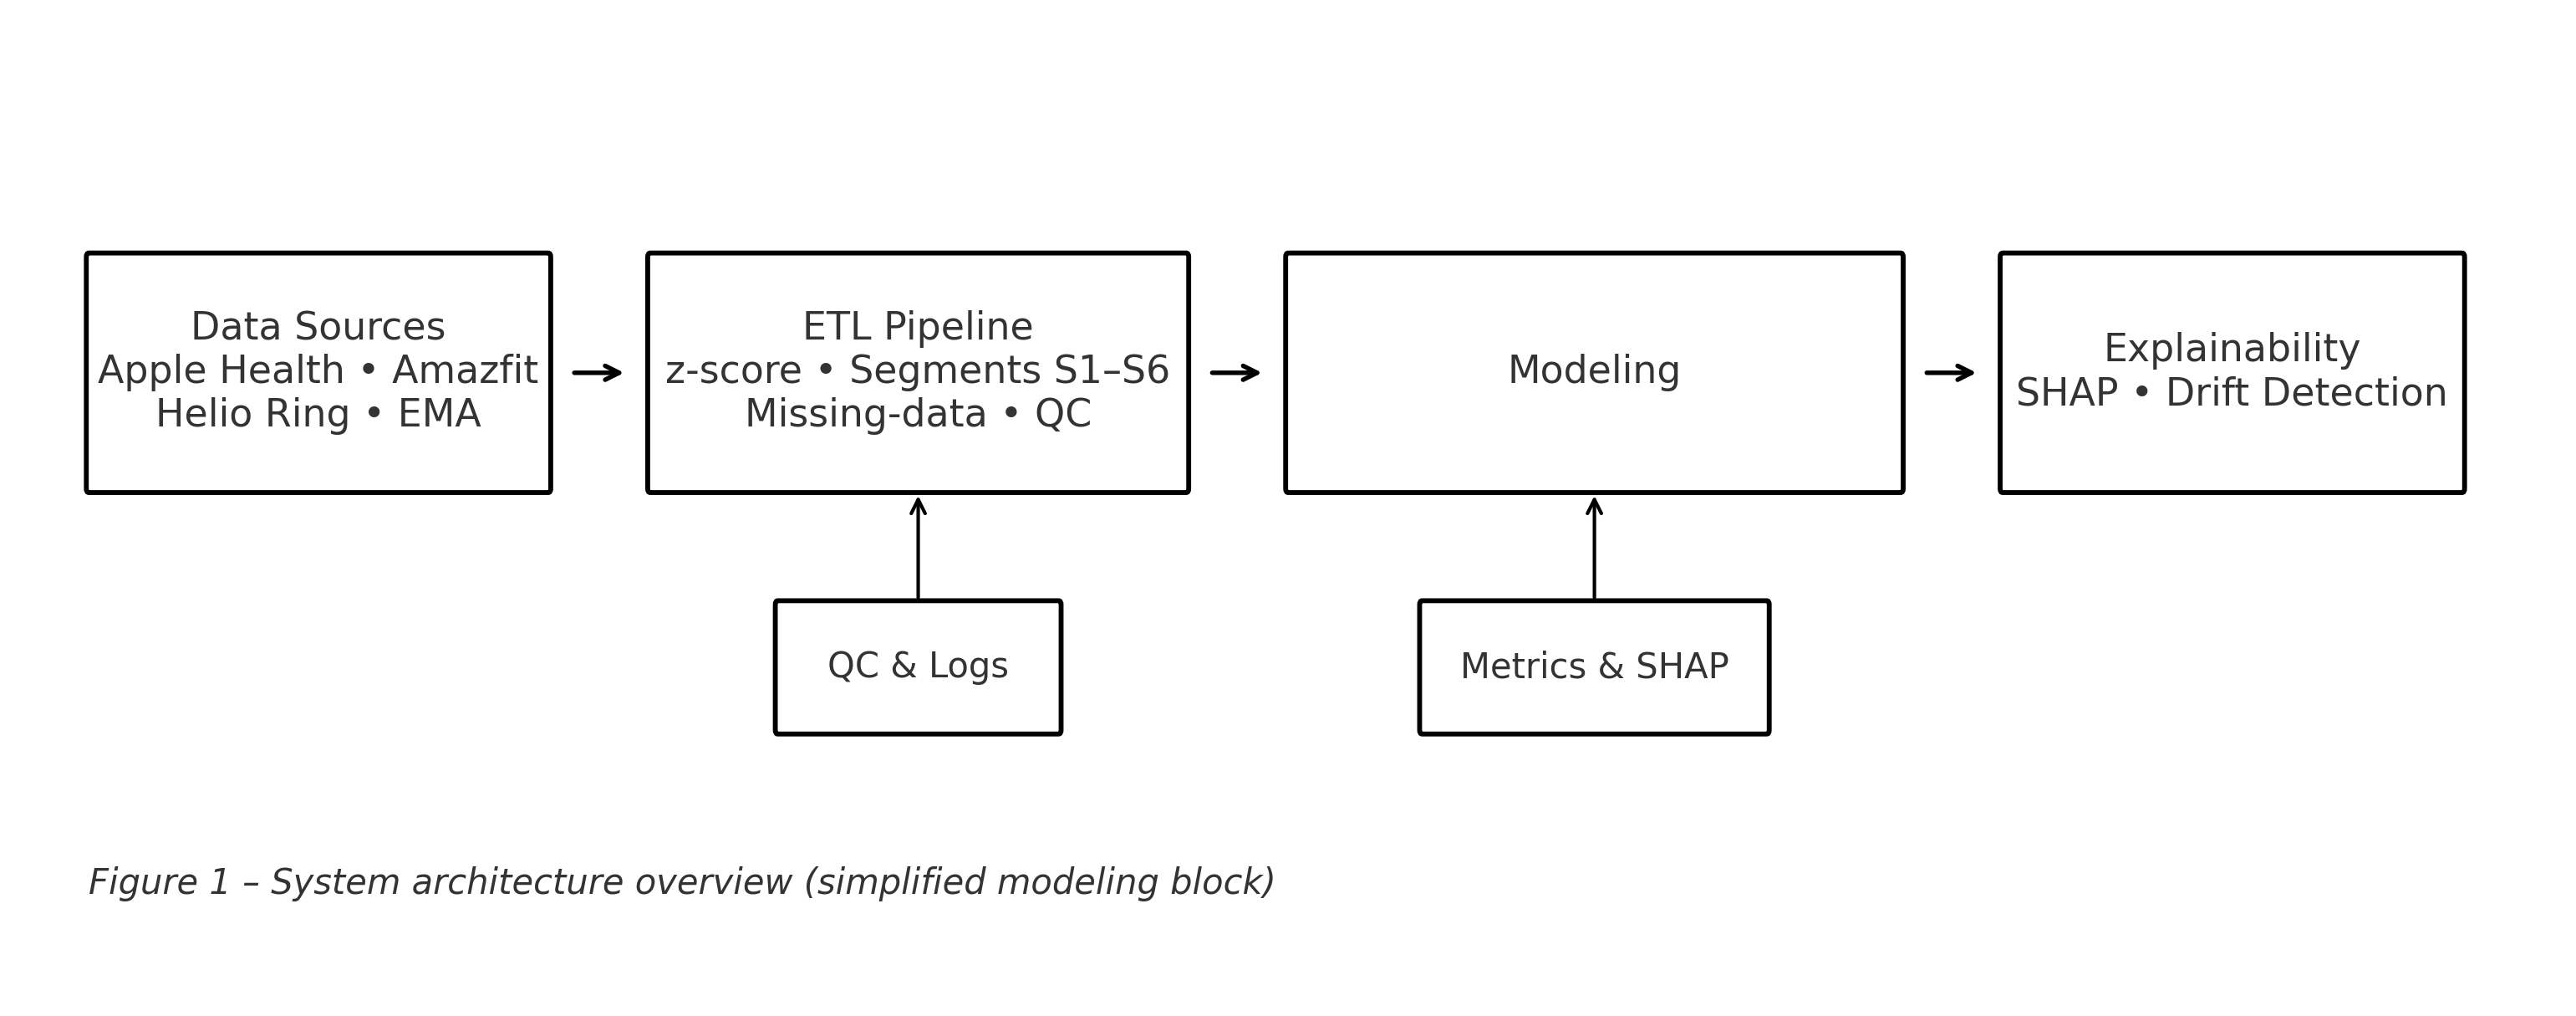
\includegraphics[width=0.9\linewidth]{docs/figures/system-architecture-paper-v3.png}
  \caption{System architecture overview with internal LSTM layers.}
  \label{fig:architecture}
\end{figure}

% ======================================================
% 3. Environment Setup
% ======================================================
\section{Environment Setup}
\subsection{Requirements}
Python 3.10+ with the dependencies listed in \texttt{requirements.txt}.

\subsection{Execution}
\begin{verbatim}
cd etl
pip install -r requirements.txt
python etl_pipeline.py
\end{verbatim}

% ======================================================
% 4. Data Management and Preprocessing
% ======================================================
\section{Data Management and Preprocessing}

The data used in this study originate from wearable and smartphone-based sensors, collected continuously over multiple months as part of an N-of-1 longitudinal experiment on ADHD and Bipolar Disorder comorbidity. 
Primary data sources include Apple Health (heart rate, heart rate variability, sleep stages, step count, screen time), Amazfit devices (heart rate and HRV), and Helio Ring (temperature and emotional state), complemented by Ecological Momentary Assessments (EMA) and Apple “State of Mind” self-reports.

All raw data are exported in CSV format and processed locally through a reproducible Python pipeline (\texttt{etl\_pipeline.py}). The ETL system is responsible for daily feature generation, data normalization, segmentation, and quality control. The overall flow is shown in Figure~\ref{fig:etl-pipeline}.

\subsection*{Normalization}
Each physiological or behavioral feature is normalized using z-score standardization, ensuring comparability across signals and devices:
\[
z_i = \frac{x_i - \mu}{\sigma}
\]
where $x_i$ is the raw value for day $i$, $\mu$ is the rolling mean, and $\sigma$ is the rolling standard deviation over a defined window.

\subsection*{Segmentation}
The dataset is divided into six temporal segments ($S_1$–$S_6$), each corresponding to distinct device firmware versions or clinical states. This segmentation supports drift analysis and model retraining in a controlled time-aware fashion.

\subsection*{Feature Extraction}
Daily-level features are aggregated from multiple raw channels (e.g., HR mean, HRV standard deviation, sleep duration, screen time, temperature variation). 
New engineered features are derived through moving averages, differences, and z-score trends, resulting in a structured dataset suitable for time-series modeling.

\subsection*{Fallback and Missing Data Handling}
In the presence of missing or inconsistent records, fallback rules are applied:
\begin{itemize}
    \item Forward-fill for short gaps ($\leq$ 1 day) in continuous data;
    \item Median replacement within the same segment for longer gaps;
    \item Removal of invalid or out-of-range values after cross-source validation.
\end{itemize}
A detailed summary of missingness and replacements is logged in \texttt{etl\_qc\_summary.csv}.

\subsection*{Outputs}
The final ETL stage produces two main outputs:
\begin{enumerate}
    \item \textbf{features\_daily.csv} – the normalized, aggregated dataset ready for modeling;
    \item \textbf{etl\_qc\_summary.csv} – a data quality and missingness report.
\end{enumerate}
These files are regenerated automatically each time the pipeline is executed, ensuring full traceability and version control.

\begin{figure}[H]
  \centering
  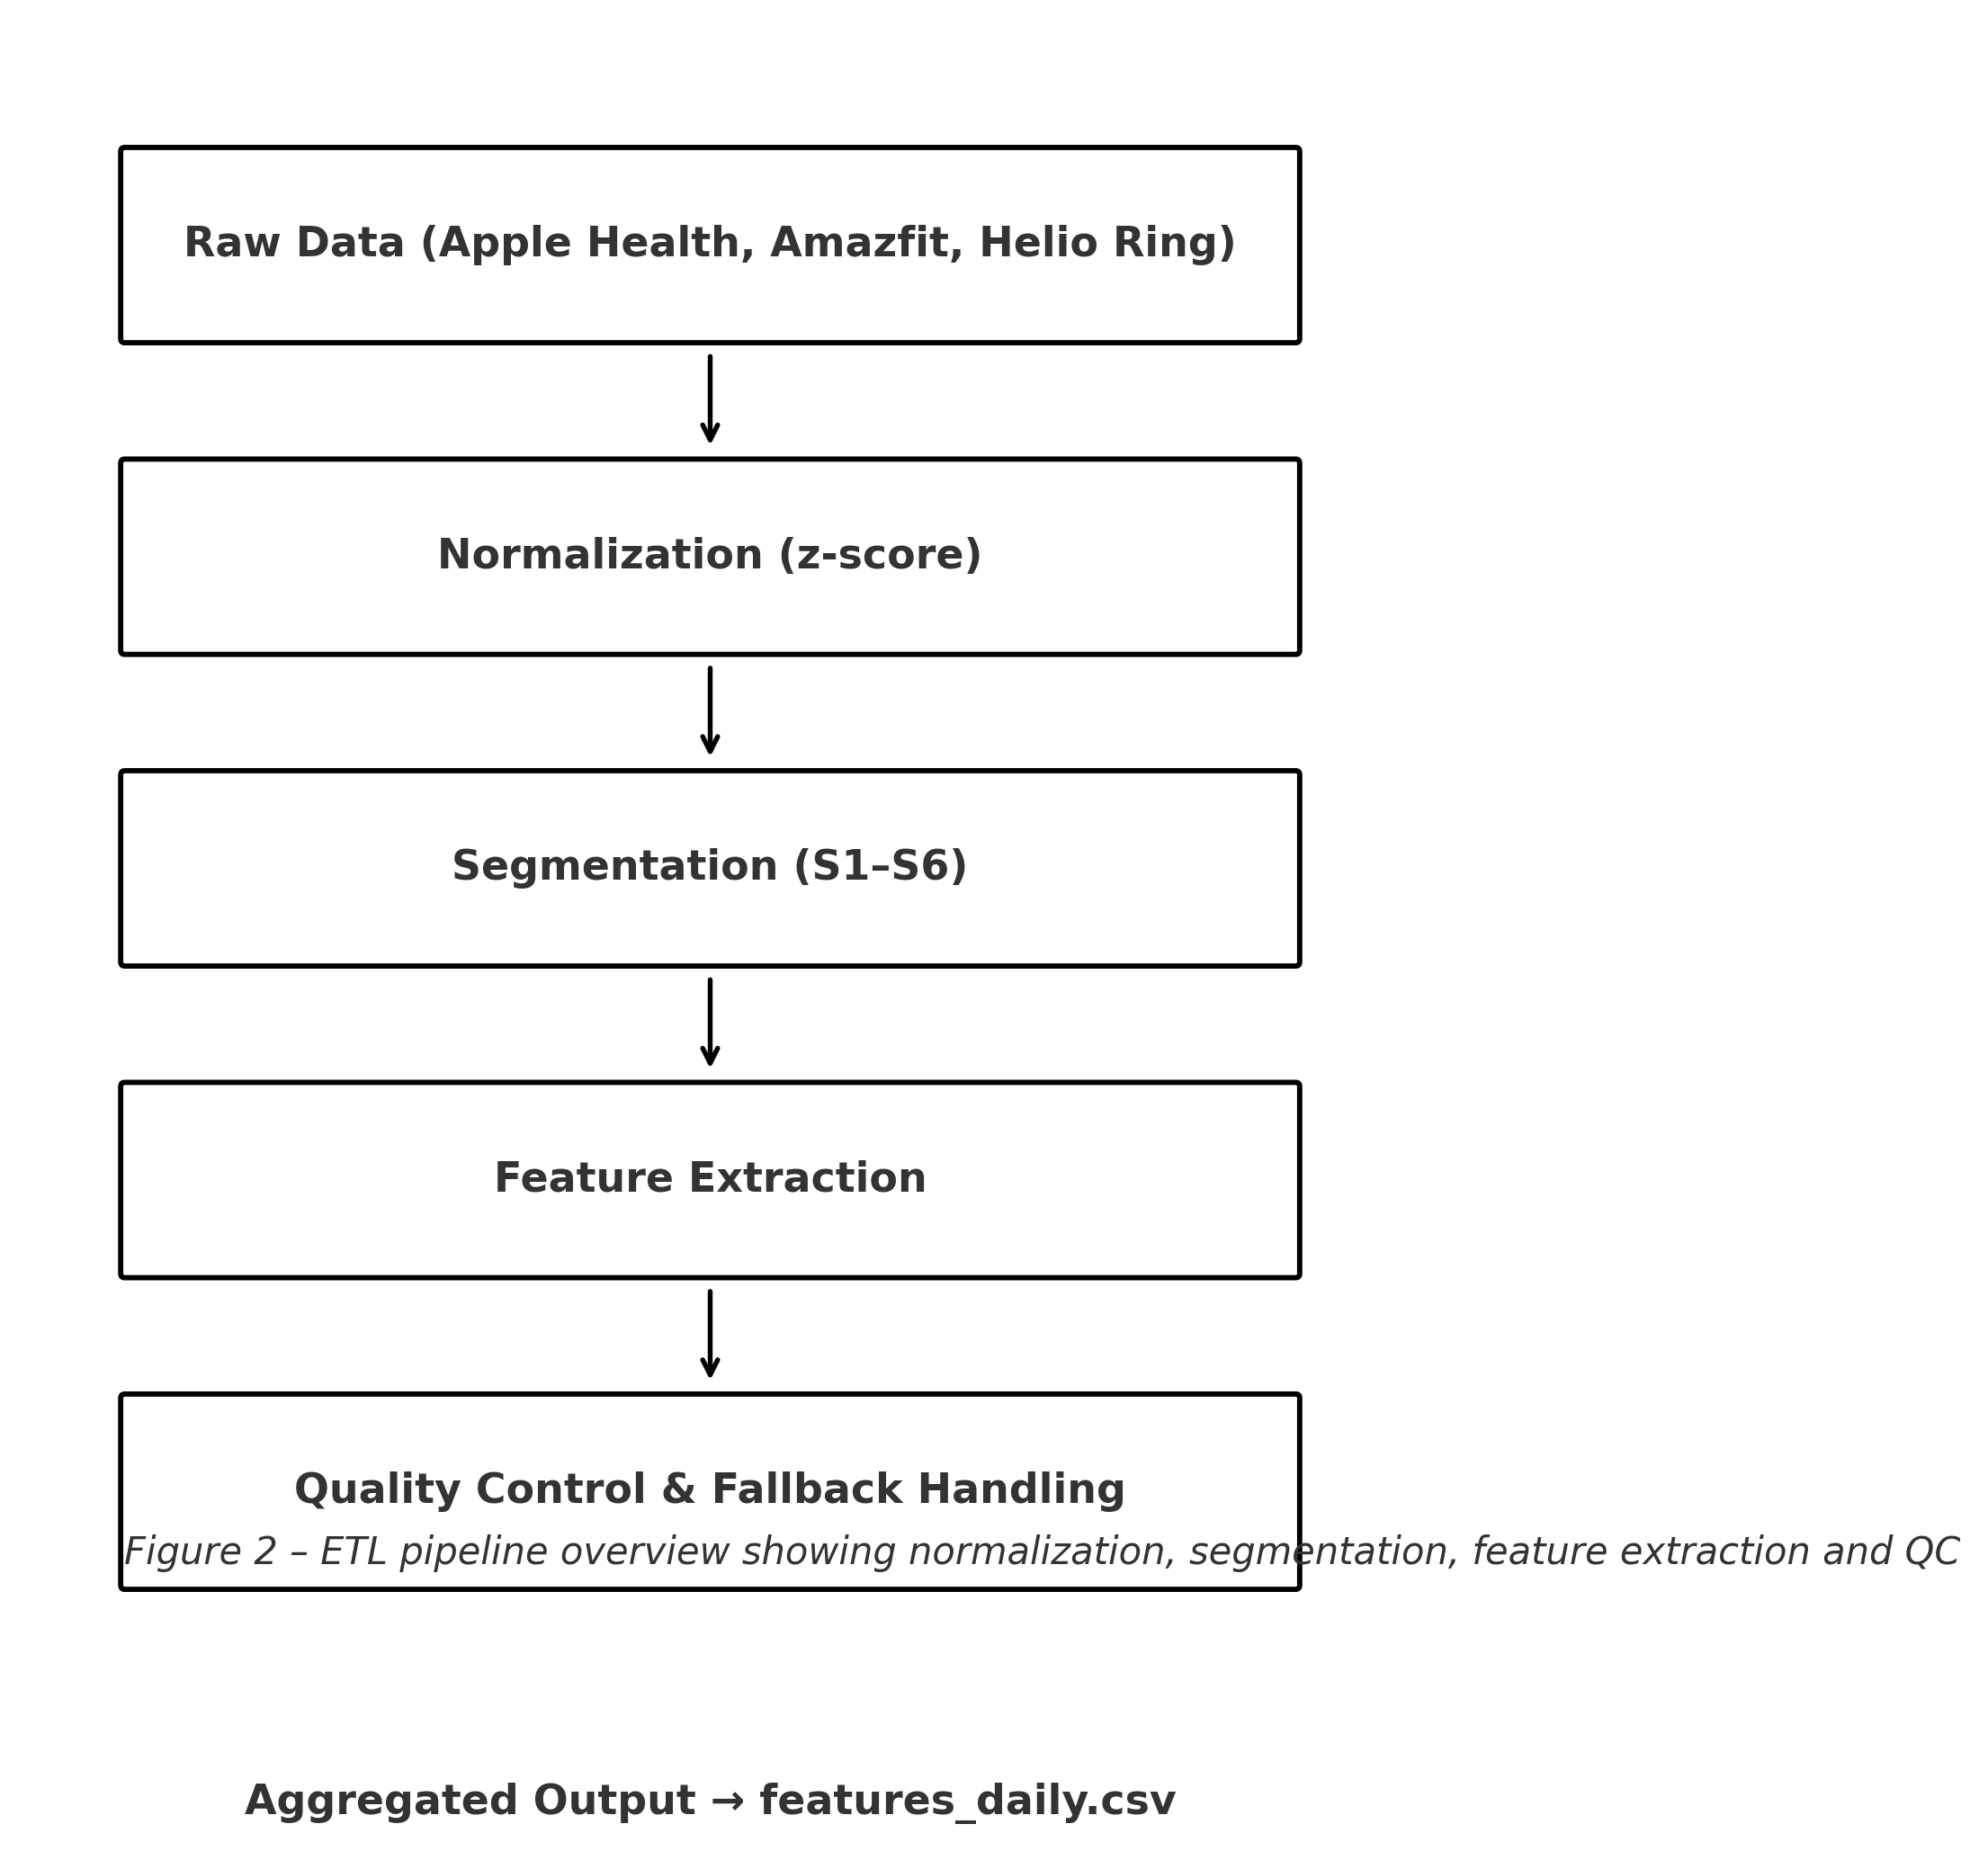
\includegraphics[width=0.75\linewidth]{docs/figures/etl-pipeline-paper.png}
  \caption{ETL pipeline overview showing normalization, segmentation, feature extraction and quality control.}
  \label{fig:etl-pipeline}
\end{figure}


% ======================================================
% 5. Modeling Framework
% ======================================================
\section{Modeling Framework}
\textbf{Notebooks:} \textit{01\_feature\_engineering.ipynb}, \textit{02\_model\_training.ipynb}, \textit{03\_shap\_analysis.ipynb}, \textit{04\_rule\_based\_baseline.ipynb}. Time-based CV uses 6 folds (4 months train / 2 months validation). Metrics: $F_1$-macro, AUROC-OvR, Balanced Accuracy, Cohen's $\kappa$, and McNemar $p$-test. The best model is exported as \texttt{best\_model.tflite}.

% ======================================================
% 6. Ethics and Governance
% ======================================================
\section{Ethics and Governance}
Phase~1: self-data. 
Phase~2: additional participants with consent and anonymisation. See documents under \texttt{docs/}.

% ======================================================
% 7. Reproducibility and Version Control
% ======================================================
\section{Reproducibility and Version Control}
The public repository contains only anonymised or synthetic samples. Version tags: \texttt{v2.0-pre-ethics}, \texttt{v2.1-ethics-approved}, \texttt{v2.2-modeling-complete}, \texttt{v2.3-final-report}.

% ======================================================
% 8. Future Work and Extensions
% ======================================================
\section{Future Work and Extensions}
Planned: S7--S9 data collection, automated drift monitoring, Helio Ring emotion via Zepp Cloud API, and clinician-backed label validation.

% ======================================================
% Appendix
% ======================================================
\appendix
\section{Appendix}
Add configuration tables, parameter grids, or pseudocode excerpts. Example inline math: $h_t = f(Wx_t + Uh_{t-1} + b)$.

\end{document}